\documentclass[11pt,a4paper]{article}

% ─── PACKAGES ──────────────────────────────────────────────────────────────────
\usepackage[utf8]{inputenc}
\usepackage[T1]{fontenc}
\usepackage{amsmath,amssymb,amsthm}
\usepackage{mathtools}
\usepackage{geometry}
\usepackage{tikz}
\usepackage{pgfplots}
\usepackage{hyperref}
\usepackage{enumitem}
\usepackage{booktabs}
\usepackage{xcolor}
\usepackage{tcolorbox}
\usepackage{microtype}
\usepackage{titlesec}

\geometry{margin=1in}
\pgfplotsset{compat=1.18}
\usetikzlibrary{arrows.meta,patterns,decorations.markings,calc}

% ─── COLORS ────────────────────────────────────────────────────────────────────
\definecolor{accent}{HTML}{e8624a}
\definecolor{accentblue}{HTML}{5b8dee}
\definecolor{accentgreen}{HTML}{52c98d}
\definecolor{gold}{HTML}{d4a84b}
\definecolor{darkbg}{HTML}{0d0d0f}
\definecolor{mutedtext}{HTML}{7a7590}

% ─── THEOREM ENVIRONMENTS ──────────────────────────────────────────────────────
\newtheorem{theorem}{Theorem}
\newtheorem{proposition}[theorem]{Proposition}
\newtheorem{lemma}[theorem]{Lemma}
\newtheorem{corollary}[theorem]{Corollary}
\newtheorem{definition}[theorem]{Definition}
\theoremstyle{remark}
\newtheorem{remark}{Remark}
\newtheorem{example}{Example}

% ─── TCOLORBOX STYLES ─────────────────────────────────────────────────────────
\tcbuselibrary{skins,breakable}

% Legacy coloured environments render as plain remarks.
\newenvironment{keyresult}{\par\medskip\noindent\textit{Remark.}\ }{\par\medskip}
\newenvironment{geometricinsight}{\par\medskip\noindent\textit{Remark.}\ }{\par\medskip}
\newenvironment{pathology}{\par\medskip\noindent\textit{Example.}\ }{\par\medskip}
\newenvironment{designprinciple}{\par\medskip\noindent\textit{Remark.}\ }{\par\medskip}

% ─── HYPERREF SETUP ────────────────────────────────────────────────────────────
\hypersetup{
  colorlinks=true,
  linkcolor=accent,
  citecolor=accentblue,
  urlcolor=accentblue
}

% ─── TITLE ─────────────────────────────────────────────────────────────────────
\title{%
  \vspace{-1cm}
  {\Large\scshape Notes on Differential Geometry in Neural Networks}\\[0.6em]
  \textbf{Manifolds, Activations, and Lost Geometry:\\
  How Pointwise Nonlinearities Break the Map}
}
\author{Taha Bouhsine\\[0.3em]{\normalsize\textit{azetta.ai}}}
\date{20 February 2026}

% ═══════════════════════════════════════════════════════════════════════════════
\begin{document}
\maketitle

% ─── ABSTRACT ──────────────────────────────────────────────────────────────────
\begin{abstract}
A neural network layer defines a map $F: \mathbb{R}^n \to \mathbb{R}^m$, and its restriction to a data manifold $M$ determines the geometry of the learned representation.
The Jacobian $\mathbf{J}_F$ controls how local distances, angles, and volumes are transported from $M$ to representation space, so the question of what each architectural choice does to geometry becomes a question about $\mathbf{J}_F$.
We analyse pointwise activation functions in this framework.
Every such activation factors the Jacobian as $\mathbf{J}_F = \mathbf{D}_\phi \mathbf{W}$, with $\mathbf{D}_\phi$ a diagonal modulation of the linear part.
Under the activations in common use, $\mathbf{D}_\phi$ admits only a narrow set of structural options: zeros (ReLU), saturating tails (sigmoid, tanh), or smooth strictly-positive entries (GELU, softplus, leaky ReLU).
Each option translates into a distinct geometric pathology---exact rank collapse, ill-conditioning, metric warping, non-injectivity---and we make the translation precise in each case.
We then identify a topological sufficient condition under which the layer preserves the manifold structure (strict monotonicity of $\phi$ together with full column rank of $\mathbf{W}$) and contrast it with the activations that fail the condition.
The analysis points to a recurring design tension we call the \emph{expressivity--geometry tradeoff}: sharper selective nonlinearities separate classes better and degrade geometric fidelity in lockstep, and no purely pointwise nonlinearity escapes the tradeoff.
\end{abstract}

% ═══════════════════════════════════════════════════════════════════════════════
\section{Introduction}
\label{sec:intro}
% ═══════════════════════════════════════════════════════════════════════════════

The manifold hypothesis~\cite{bengio2013manifold}---that high-dimensional data concentrates near a much lower-dimensional submanifold $M \subset \mathbb{R}^D$---has become a foundational working assumption in deep learning.
Under the hypothesis, the network's task is not to fit a function on all of $\mathbb{R}^D$ but to learn a \emph{map from the data manifold into a representation space}: $M \to N \subset \mathbb{R}^m$, where the downstream task becomes simple.

The quality of this map is governed by its Jacobian.
A well-behaved Jacobian preserves local geometry: nearby points stay nearby, angles between tangent vectors are approximately maintained, and local volumes do not collapse.
A degenerate Jacobian destroys local geometry, and the loss is irreversible---the next layer cannot recover what this one collapsed.

Not all geometric distortion is harmful.
Collapsing nuisance directions---directions that carry no task-relevant information---is in fact useful: it reduces the effective dimensionality of the representation to what matters.
The point of the analysis is therefore not that activations should preserve all geometry, but that one should know which geometric structure is being preserved and which is being thrown away.
The analysis below characterises \emph{what} activations do to geometry; whether a particular distortion helps or hurts is a task-level judgement.

We focus on the specific mechanism by which geometry is degraded or destroyed in practice: \textbf{pointwise activation functions}.
Every standard activation---ReLU, sigmoid, tanh, GELU, softplus---acts coordinatewise on the pre-activation vector $\mathbf{z} = \mathbf{W}\mathbf{x} + \mathbf{b}$, and this single fact forces the Jacobian to factor as $\mathbf{J}_F = \mathbf{D}_\phi \mathbf{W}$, with $\mathbf{D}_\phi$ a diagonal matrix of activation derivatives.
The diagonal factor is therefore the activation's entire geometric contribution.
When entries of $\mathbf{D}_\phi$ vanish (as in ReLU), $\mathbf{J}_F$ can lose rank exactly and collapse directions of the data manifold onto a lower-dimensional subset of representation space.
When entries of $\mathbf{D}_\phi$ approach zero without vanishing (as in sigmoid or tanh), the Jacobian remains full-rank in the strict sense but its condition number grows, local volumes shrink toward zero, and the effective dimension of the representation degrades.

The paper is organised as follows.
Section~\ref{sec:prelim} fixes notation and recalls the manifold hypothesis.
Section~\ref{sec:jacobian} states the factorisation $\mathbf{J}_F = \mathbf{D}_\phi \mathbf{W}$ and records its consequences for rank, conditioning, and the pullback metric.
Section~\ref{sec:activations} analyses each standard activation in this framework.
Section~\ref{sec:topology} gives a sufficient condition---strict monotonicity of $\phi$ together with full column rank of $\mathbf{W}$---under which the layer restricted to a compact data manifold is a homeomorphism, and treats the pullback metric in the same setting.
Section~\ref{sec:highdim} records a high-dimensional scaling result for ReLU.
Section~\ref{sec:tradeoff} is the discussion section.
We frame the \emph{expressivity--geometry tradeoff} there as a conjectural design principle rather than as a theorem, together with the deeper Riemannian reading of the layer as a representation; that material is offered as motivation and consequence rather than as further mathematical content.

% ═══════════════════════════════════════════════════════════════════════════════
\section{Preliminaries: Manifolds and Maps}
\label{sec:prelim}
% ═══════════════════════════════════════════════════════════════════════════════

\subsection{The Manifold Hypothesis}

\begin{definition}[Data manifold]
\label{def:data-manifold}
A \emph{data manifold} is a compact, connected, smooth submanifold $M \hookrightarrow \mathbb{R}^D$ of intrinsic dimension $d \ll D$, such that the data distribution $p$ has its support concentrated on or near $M$:
\[
  \mathrm{supp}(p) \subseteq M_\varepsilon \coloneqq \{\mathbf{x} \in \mathbb{R}^D : \mathrm{dist}(\mathbf{x}, M) < \varepsilon\}
\]
for some small $\varepsilon > 0$.
\end{definition}

The manifold hypothesis asserts that natural data (images, text, speech) typically lies on such an $M$, even though each datum is represented as a vector in $\mathbb{R}^D$ with $D$ potentially in the millions.
The intrinsic dimension $d$ is the geometric content the network must preserve; the ambient dimension $D$ is incidental.

\subsection{Neural Network Layers as Smooth Maps}

A single layer of a neural network, including its activation function, defines a map:
\begin{equation}
  F: \mathbb{R}^n \to \mathbb{R}^m, \qquad F(\mathbf{x}) = \phi(\mathbf{W}\mathbf{x} + \mathbf{b}),
  \label{eq:layer}
\end{equation}
where $\mathbf{W} \in \mathbb{R}^{m \times n}$, $\mathbf{b} \in \mathbb{R}^m$, and $\phi: \mathbb{R} \to \mathbb{R}$ is applied coordinatewise:
$\phi(\mathbf{z})_i = \phi(z_i)$.

When restricted to the data manifold $M$, $F$ becomes a map $F|_M: M \to N$, where $N = F(M)$ is the \emph{representation image}.
When $F|_M$ is a smooth immersion (in particular, when $\mathbf{J}_F$ has full column rank everywhere on $M$), $N$ inherits a smooth manifold structure; otherwise, $N$ may be a lower-dimensional or singular subset of $\mathbb{R}^m$.

\begin{definition}[Pullback metric]
\label{def:pullback}
Let $(N, g_N)$ be a Riemannian manifold and $F: M \to N$ a smooth map.
The \emph{pullback metric} on $M$ is the tensor:
\begin{equation}
  (F^* g_N)(\mathbf{u}, \mathbf{v}) = g_N\bigl(\mathbf{J}_F \cdot \mathbf{u},\; \mathbf{J}_F \cdot \mathbf{v}\bigr) \qquad \text{for } \mathbf{u}, \mathbf{v} \in T_{\mathbf{x}} M,
  \label{eq:pullback}
\end{equation}
or in matrix form: $g_M = \mathbf{J}_F^\top \, g_N \, \mathbf{J}_F$.
\end{definition}

The pullback metric encodes how $F$ stretches, compresses, and rotates tangent vectors.
If $g_N$ is the standard Euclidean metric ($g_N = \mathbf{I}$), then $g_M = \mathbf{J}_F^\top \mathbf{J}_F$, and local distances in data space are governed entirely by the singular values of $\mathbf{J}_F$.

% ═══════════════════════════════════════════════════════════════════════════════
\section{The Jacobian of a Layer with Activations}
\label{sec:jacobian}
% ═══════════════════════════════════════════════════════════════════════════════

\subsection{Diagonal Structure}

\begin{remark}[Scope: ambient analysis]
\label{rem:scope}
The data manifold $M$ has intrinsic dimension $d$, and the geometrically correct object is the restricted differential $d(F|_M)_{\mathbf{x}}: T_{\mathbf{x}}M \to T_{F(\mathbf{x})}\mathbb{R}^m$.
However, since $T_{\mathbf{x}}M \subset \mathbb{R}^n$, the restricted differential is the composition of the ambient Jacobian $\mathbf{J}_F(\mathbf{x})$ with the inclusion of $T_{\mathbf{x}}M$.
For clarity, we analyze the ambient Jacobian $\mathbf{J}_F \in \mathbb{R}^{m \times n}$ throughout; the ambient Jacobian constrains what the restricted map $F|_M$ can preserve, but the actual behavior on $M$ depends on how the tangent space $T_{\mathbf{x}}M$ sits relative to the singular directions and kernel of $\mathbf{J}_F(\mathbf{x})$.
If $\mathbf{J}_F$ has full column rank, then $d(F|_M)_{\mathbf{x}}$ is injective on $T_{\mathbf{x}}M$ for any $d$-dimensional $M$.
If $\mathbf{J}_F$ is rank-deficient, the restriction to $T_{\mathbf{x}}M$ may or may not lose rank depending on the alignment of $T_{\mathbf{x}}M$ with the kernel.
\end{remark}

The structural fact that drives everything below is that pointwise activations contribute a \emph{diagonal} factor to the Jacobian, and only a diagonal factor.

\begin{proposition}[Layer Jacobian]
\label{prop:jacobian}
For the layer $F(\mathbf{x}) = \phi(\mathbf{W}\mathbf{x} + \mathbf{b})$ with $\phi$ applied coordinatewise, the Jacobian at $\mathbf{x}$ is:
\begin{equation}
  \mathbf{J}_F(\mathbf{x}) = \mathbf{D}_\phi(\mathbf{z}) \cdot \mathbf{W}, \qquad \mathbf{z} = \mathbf{W}\mathbf{x} + \mathbf{b},
  \label{eq:jacobian}
\end{equation}
where $\mathbf{D}_\phi(\mathbf{z}) = \mathrm{diag}\bigl(\phi'(z_1), \phi'(z_2), \dots, \phi'(z_m)\bigr)$ is the diagonal matrix of activation derivatives.
\end{proposition}

\begin{proof}
By the chain rule, $\frac{\partial F_i}{\partial x_j} = \phi'(z_i) \cdot \mathbf{W}_{ij}$, which in matrix form is $\mathbf{J}_F = \mathbf{D}_\phi \cdot \mathbf{W}$.
\end{proof}

\begin{geometricinsight}
The Jacobian $\mathbf{J}_F = \mathbf{D}_\phi \cdot \mathbf{W}$ factors the layer's geometric action into two parts:
\begin{enumerate}[label=(\alph*)]
  \item $\mathbf{W}$: a linear map that rotates and scales tangent vectors (the ``learned geometry'').
  \item $\mathbf{D}_\phi$: a diagonal rescaling that selectively amplifies or suppresses each coordinate (the ``activation geometry'').
\end{enumerate}
The activation does not create new geometric structure---it can only \emph{modulate} what the linear part provides.
\end{geometricinsight}

\subsection{Rank, Singular Values, and Volume}

\begin{definition}[Effective rank]
\label{def:effective-rank}
The \emph{effective rank} of $\mathbf{J}_F$ at a point $\mathbf{x}$ is the number of singular values $\sigma_i(\mathbf{J}_F(\mathbf{x}))$ that exceed a threshold $\varepsilon > 0$.
For pointwise activations:
\begin{equation}
  \operatorname{rank}_\varepsilon(\mathbf{J}_F(\mathbf{x})) = \operatorname{rank}_\varepsilon(\mathbf{D}_\phi(\mathbf{z}) \cdot \mathbf{W}) \leq \min\bigl(\operatorname{rank}(\mathbf{W}),\; |\{i : |\phi'(z_i)| > \varepsilon\}|\bigr).
  \label{eq:effective-rank}
\end{equation}
\end{definition}

\begin{proposition}[Volume element]
\label{prop:volume}
Let $F(\mathbf{x}) = \phi(\mathbf{W}\mathbf{x} + \mathbf{b})$ with $\mathbf{W} \in \mathbb{R}^{m \times n}$.
The local $n$-dimensional volume scaling factor of the ambient map (measuring how $F$ scales infinitesimal $n$-dimensional parallelepipeds) is:
\begin{equation}
  \mathrm{vol}_n(\mathbf{J}_F) = \sqrt{\det(\mathbf{J}_F^\top \mathbf{J}_F)} = \sqrt{\det(\mathbf{W}^\top \mathbf{D}_\phi^2 \mathbf{W})}.
  \label{eq:volume}
\end{equation}
Here $\mathbf{J}_F^\top \mathbf{J}_F \in \mathbb{R}^{n \times n}$, so the Gram determinant is well-defined regardless of whether $m = n$ or $m > n$.

In the special case $m = n$, this simplifies to $|\det(\mathbf{D}_\phi)| \cdot |\det(\mathbf{W})| = \bigl(\prod_{i=1}^m |\phi'(z_i)|\bigr) |\det(\mathbf{W})|$.
For general $m \geq n$: if any $\phi'(z_i) = 0$, the corresponding row of $\mathbf{J}_F = \mathbf{D}_\phi \mathbf{W}$ is zeroed, reducing the row space.
When sufficiently many rows are zeroed that $\operatorname{rank}(\mathbf{J}_F) < n$, the Gram determinant vanishes: the map squashes a neighborhood of $\mathbf{x}$ to a set of dimension less than $n$.
For saturating activations where $\phi'(z_i) \to 0$ without reaching zero, the Gram determinant approaches (but does not reach) zero---the volume shrinks but does not exactly collapse.

When $M$ has intrinsic dimension $d < n$, the relevant quantity is the $d$-dimensional volume element on $T_{\mathbf{x}}M$, which depends on the restriction of $\mathbf{J}_F$ to $T_{\mathbf{x}}M$ rather than on $\mathbf{J}_F$ alone (see Remark~\ref{rem:scope}).
\end{proposition}

\begin{figure}[ht]
\centering
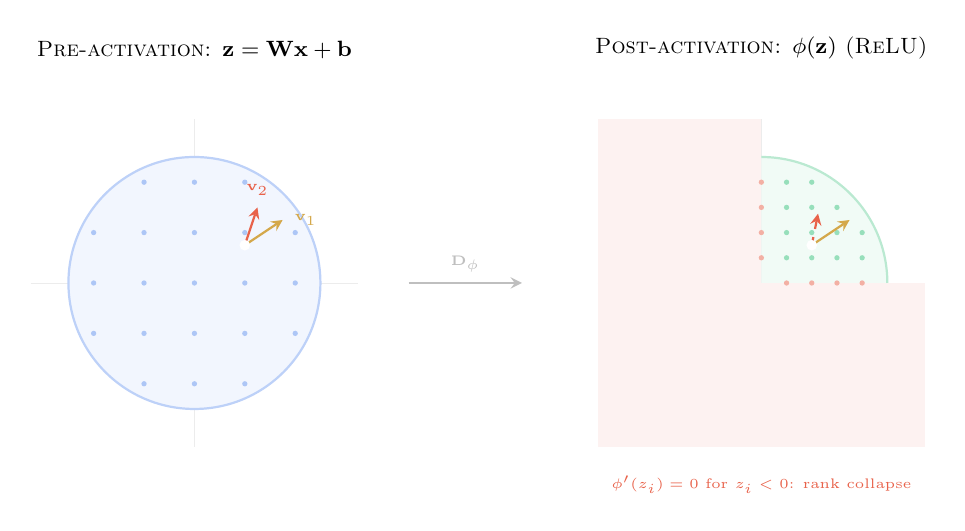
\begin{tikzpicture}[scale=1.6]
  % ── LEFT: Before activation ──
  \begin{scope}[shift={(-3,0)}]
    \node[font=\footnotesize\scshape, anchor=south] at (0,1.7) {Pre-activation: $\mathbf{z} = \mathbf{W}\mathbf{x} + \mathbf{b}$};

    % Grid
    \draw[gray!15, very thin] (-1.3,0) -- (1.3,0);
    \draw[gray!15, very thin] (0,-1.3) -- (0,1.3);

    % Disk
    \fill[accentblue!8] (0,0) circle (1);
    \draw[accentblue!40, thick] (0,0) circle (1);

    % Grid points
    \foreach \i in {-0.8,-0.4,0,0.4,0.8} {
      \foreach \j in {-0.8,-0.4,0,0.4,0.8} {
        \pgfmathparse{sqrt(\i*\i+\j*\j) < 1 ? 1 : 0}
        \ifnum\pgfmathresult=1
          \fill[accentblue!50] (\i,\j) circle (0.6pt);
        \fi
      }
    }

    % Tangent vectors
    \draw[gold, thick, ->, >=stealth] (0.4,0.3) -- (0.7,0.5);
    \draw[accent, thick, ->, >=stealth] (0.4,0.3) -- (0.5,0.6);
    \fill[white] (0.4,0.3) circle (1.2pt);

    \node[font=\tiny, text=gold, anchor=west] at (0.72,0.5) {$\mathbf{v}_1$};
    \node[font=\tiny, text=accent, anchor=south] at (0.5,0.62) {$\mathbf{v}_2$};
  \end{scope}

  % ── Arrow ──
  \draw[thick, ->, >=stealth, gray!50] (-1.3,0) -- (-0.4,0) node[midway, above, font=\tiny] {$\mathbf{D}_\phi$};

  % ── RIGHT: After ReLU ──
  \begin{scope}[shift={(1.5,0)}]
    \node[font=\footnotesize\scshape, anchor=south] at (0,1.7) {Post-activation: $\phi(\mathbf{z})$ (ReLU)};

    % Grid
    \draw[gray!15, very thin] (-1.3,0) -- (1.3,0);
    \draw[gray!15, very thin] (0,-1.3) -- (0,1.3);

    % Collapsed region (negative quadrants)
    \fill[accent!8] (-1.3,-1.3) rectangle (0,1.3);
    \fill[accent!8] (-1.3,-1.3) rectangle (1.3,0);

    % Surviving quadrant
    \fill[accentgreen!8] (0,0) -- (1,0) arc (0:90:1) -- cycle;
    \draw[accentgreen!40, thick] (1,0) arc (0:90:1);

    % Collapsed points on axes
    \foreach \j in {0.2,0.4,0.6,0.8} {
      \fill[accent!50] (0,\j) circle (0.6pt);
      \fill[accent!50] (\j,0) circle (0.6pt);
    }

    % Surviving grid points
    \foreach \i in {0.2,0.4,0.6,0.8} {
      \foreach \j in {0.2,0.4,0.6,0.8} {
        \pgfmathparse{sqrt(\i*\i+\j*\j) < 1 ? 1 : 0}
        \ifnum\pgfmathresult=1
          \fill[accentgreen!60] (\i,\j) circle (0.6pt);
        \fi
      }
    }

    % Tangent vectors (one collapsed)
    \draw[gold, thick, ->, >=stealth] (0.4,0.3) -- (0.7,0.5);
    \draw[accent, thick, ->, >=stealth, dashed] (0.4,0.3) -- (0.45,0.55);
    \fill[white] (0.4,0.3) circle (1.2pt);

    % Rank label
    \node[font=\tiny, text=accent, anchor=north] at (0,-1.45) {$\phi'(z_i) = 0$ for $z_i < 0$: rank collapse};
  \end{scope}
\end{tikzpicture}
\caption{Schematic: a 2D disk before and after ReLU.
\textbf{Left:} The pre-activation space with two tangent vectors $\mathbf{v}_1, \mathbf{v}_2$ at a point.
\textbf{Right:} After ReLU, the negative quadrants collapse onto the axes.
The \textcolor{accent}{red shaded region} maps to zero; the \textcolor{accentgreen}{green quarter-disk} survives.
Tangent vector directions into the collapsed region are lost.}
\label{fig:relu-collapse}
\end{figure}

% ═══════════════════════════════════════════════════════════════════════════════
\section{Activation Functions as Geometric Operators}
\label{sec:activations}
% ═══════════════════════════════════════════════════════════════════════════════

We now analyze each standard activation through the lens of the Jacobian framework.
For each activation $\phi$, we characterize: (1) the derivative $\phi'$ and its range, (2) whether exact rank collapse or ill-conditioning occurs (and where), and (3) the metric distortion.

\subsection{Linear (Identity)}

\begin{definition}
$\phi(x) = x$, so $\phi'(x) = 1$ everywhere.
\end{definition}

\begin{proposition}
With the identity activation, $\mathbf{D}_\phi = \mathbf{I}$ and $\mathbf{J}_F = \mathbf{W}$.  The layer is a pure linear map: it preserves rank, invertibility is determined solely by $\mathbf{W}$, and the pullback metric is $g_M = \mathbf{W}^\top \mathbf{W}$.  No saturation, no collapse.
\end{proposition}

This is the baseline: no expressivity beyond linearity, but perfect geometric fidelity.

\subsection{ReLU}

\begin{definition}
$\phi(x) = \max(0, x)$, so $\phi'(x) = \mathbf{1}_{x > 0}$ (with $\phi'(0)$ undefined or set to 0).
\end{definition}

\begin{theorem}[ReLU rank collapse]
\label{thm:relu-collapse}
Let $F(\mathbf{x}) = \mathrm{ReLU}(\mathbf{W}\mathbf{x} + \mathbf{b})$ and let $S(\mathbf{x}) = \{i : (\mathbf{W}\mathbf{x}+\mathbf{b})_i > 0\}$ be the set of active neurons.
Then:
\begin{equation}
  \operatorname{rank}(\mathbf{J}_F(\mathbf{x})) = \operatorname{rank}(\mathbf{W}_{S(\mathbf{x}), :}),
  \label{eq:relu-rank}
\end{equation}
where $\mathbf{W}_{S(\mathbf{x}),:}$ is the submatrix of $\mathbf{W}$ consisting of rows indexed by $S(\mathbf{x})$.
\end{theorem}

\begin{proof}
$\mathbf{D}_\phi = \mathrm{diag}(\mathbf{1}_{z_i > 0})$ zeros out entire rows of $\mathbf{J}_F = \mathbf{D}_\phi \mathbf{W}$ for each $i \notin S(\mathbf{x})$.
The remaining rows are exactly $\mathbf{W}_{S(\mathbf{x}),:}$.
\end{proof}

\begin{pathology}
ReLU creates \emph{dead zones}: for any $\mathbf{x}$ such that $z_i \leq 0$, the $i$-th output coordinate is identically zero, and the corresponding row of $\mathbf{J}_F$ vanishes.
The map is piecewise linear with different ranks in different regions.
\begin{itemize}
  \item \textbf{Non-invertibility:} ReLU is coordinatewise many-to-one: any two pre-activations that differ only in coordinates where both are negative produce the same output, since both are mapped to zero in those coordinates.
  \item \textbf{Volume collapse:} $\mathrm{vol}_n(\mathbf{J}_F) = 0$ whenever $\operatorname{rank}(\mathbf{W}_{S(\mathbf{x}),:}) < n$, i.e., when zeroing inactive rows drops $\mathbf{J}_F$ below full column rank.
  \item \textbf{Information loss:} The map loses sensitivity to input perturbations lying in directions annihilated by the surviving row submatrix $\mathbf{W}_{S(\mathbf{x}),:}$.
\end{itemize}
\end{pathology}

\subsection{Leaky ReLU}

\begin{definition}
$\phi(x) = x$ for $x \geq 0$, $\phi(x) = \alpha x$ for $x < 0$, with $\alpha \in (0, 1)$ (typically $\alpha = 0.01$).
So $\phi'(x) = 1$ for $x > 0$ and $\phi'(x) = \alpha$ for $x < 0$.
\end{definition}

\begin{proposition}[Leaky ReLU preserves rank]
\label{prop:leaky-rank}
Since $\phi'(x) \in \{\alpha, 1\}$ with $\alpha > 0$, we have $\mathbf{D}_\phi = \mathrm{diag}(d_1, \dots, d_m)$ with every $d_i \geq \alpha > 0$.
Therefore:
\[
  \operatorname{rank}(\mathbf{J}_F) = \operatorname{rank}(\mathbf{W}).
\]
The Jacobian never loses rank due to the activation.  However, the condition number is amplified:
\begin{equation}
  \kappa(\mathbf{J}_F) \leq \frac{1}{\alpha} \cdot \kappa(\mathbf{W}),
  \label{eq:leaky-cond}
\end{equation}
so for $\alpha = 0.01$, the conditioning can worsen by a factor of 100.
To see this (assuming $\mathbf{W}$ has full column rank), note that all singular values of $\mathbf{D}_\phi$ lie in $[\alpha, 1]$, so $\sigma_{\min}(\mathbf{D}_\phi) \geq \alpha$ and $\sigma_{\max}(\mathbf{D}_\phi) \leq 1$.
For the product $\mathbf{J}_F = \mathbf{D}_\phi \mathbf{W}$:
\[
  \sigma_{\max}(\mathbf{J}_F) \leq \sigma_{\max}(\mathbf{D}_\phi) \cdot \sigma_{\max}(\mathbf{W}) \leq \sigma_{\max}(\mathbf{W}),
\]
\[
  \sigma_{\min}(\mathbf{J}_F) \geq \sigma_{\min}(\mathbf{D}_\phi) \cdot \sigma_{\min}(\mathbf{W}) \geq \alpha \cdot \sigma_{\min}(\mathbf{W}),
\]
where the second inequality uses the general fact that $\sigma_{\min}(AB) \geq \sigma_{\min}(A)\,\sigma_{\min}(B)$ when $A$ is square and nonsingular.
Hence $\kappa(\mathbf{J}_F) = \sigma_{\max}(\mathbf{J}_F)/\sigma_{\min}(\mathbf{J}_F) \leq \kappa(\mathbf{W})/\alpha$.
\end{proposition}

\subsection{Sigmoid}

\begin{definition}
$\sigma(x) = 1/(1 + e^{-x})$, so $\sigma'(x) = \sigma(x)(1 - \sigma(x))$.
\end{definition}

\begin{proposition}[Sigmoid saturation]
\label{prop:sigmoid-sat}
The derivative satisfies $\sigma'(x) \in (0, 1/4]$, with:
\begin{itemize}
  \item $\sigma'(x) \to 0$ exponentially as $|x| \to \infty$ (saturation in both tails),
  \item $\sigma'(0) = 1/4$ (maximum sensitivity at the origin).
\end{itemize}
For the layer Jacobian $\mathbf{J}_F = \mathbf{D}_\sigma \mathbf{W}$, the maximum singular value is bounded:
\begin{equation}
  \sigma_{\max}(\mathbf{J}_F) \leq \frac{1}{4} \cdot \sigma_{\max}(\mathbf{W}).
  \label{eq:sigmoid-bound}
\end{equation}
As input magnitudes grow, all diagonal entries of $\mathbf{D}_\sigma$ approach zero and $\mathbf{J}_F \to 0$: the map ``freezes'' and the representation becomes increasingly ill-conditioned, concentrating near the boundary corners of $[0,1]^m$ determined by the sign pattern of the pre-activations $\mathbf{z} = \mathbf{W}\mathbf{x} + \mathbf{b}$.
Note that $\sigma'(x) > 0$ everywhere, so \emph{exact} rank collapse never occurs---the pathology is one of conditioning, not rank.
\end{proposition}

\subsection{Tanh}

\begin{definition}
$\tanh(x) = (e^x - e^{-x})/(e^x + e^{-x})$, so $\tanh'(x) = 1 - \tanh^2(x)$.
\end{definition}

\begin{proposition}[Tanh saturation]
$\tanh'(x) \in (0, 1]$, with $\tanh'(0) = 1$ (locally identity) and $\tanh'(x) \to 0$ as $|x| \to \infty$.
The same saturation pathology as sigmoid, but centered on the origin: the output is bounded in $(-1, 1)^m$.
As with sigmoid, exact rank is preserved ($\tanh'(x) > 0$ everywhere), but the Jacobian becomes arbitrarily ill-conditioned as inputs grow.
\end{proposition}

\subsection{Softplus}

\begin{definition}
$\phi(x) = \log(1 + e^x)$, so $\phi'(x) = \sigma(x) = 1/(1 + e^{-x})$.
\end{definition}

\begin{proposition}[Softplus: smooth ReLU]
\label{prop:softplus}
Softplus is strictly monotone with $\phi'(x) = \sigma(x) \in (0, 1)$.
The derivative is strictly positive everywhere, so:
\[
  \operatorname{rank}(\mathbf{J}_F) = \operatorname{rank}(\mathbf{W}) \quad \text{at every point}.
\]
Moreover, $\phi'(x) \to 1$ for $x \to +\infty$ (linear regime) and $\phi'(x) \to 0^+$ for $x \to -\infty$ (compression but not collapse).
\end{proposition}

\subsection{GELU}

\begin{definition}
The Gaussian error linear unit~\cite{hendrycks2016gelu} is $\mathrm{GELU}(x) = x \cdot \Phi(x)$, where $\Phi$ is the CDF of $\mathcal{N}(0,1)$.
The derivative is $\mathrm{GELU}'(x) = \Phi(x) + x \cdot \varphi(x)$, where $\varphi$ is the PDF of $\mathcal{N}(0,1)$.
\end{definition}

\begin{proposition}[GELU properties]
\label{prop:gelu}
GELU is smooth, and:
\begin{itemize}
  \item $\mathrm{GELU}'(0) = 0.5$ (half-gate at origin),
  \item $\mathrm{GELU}'(x) \to 1$ as $x \to +\infty$ (approaches identity),
  \item $\mathrm{GELU}'(x) \to 0$ as $x \to -\infty$ (soft suppression),
  \item $\mathrm{GELU}'(x) > 0$ for all $x$ above the unique minimum of $\mathrm{GELU}'$.
\end{itemize}
GELU is not globally monotone: $\mathrm{GELU}'$ becomes slightly negative on a bounded interval of negative inputs, with a shallow minimum around $x \approx -1.4$ where $\mathrm{GELU}' \approx -0.13$.
Empirically, trained networks tend not to have large concentrations of pre-activations in this narrow non-monotone region, though we are not aware of a formal result establishing this.
\end{proposition}

\subsection{Comparison}

\begin{figure}[ht]
\centering
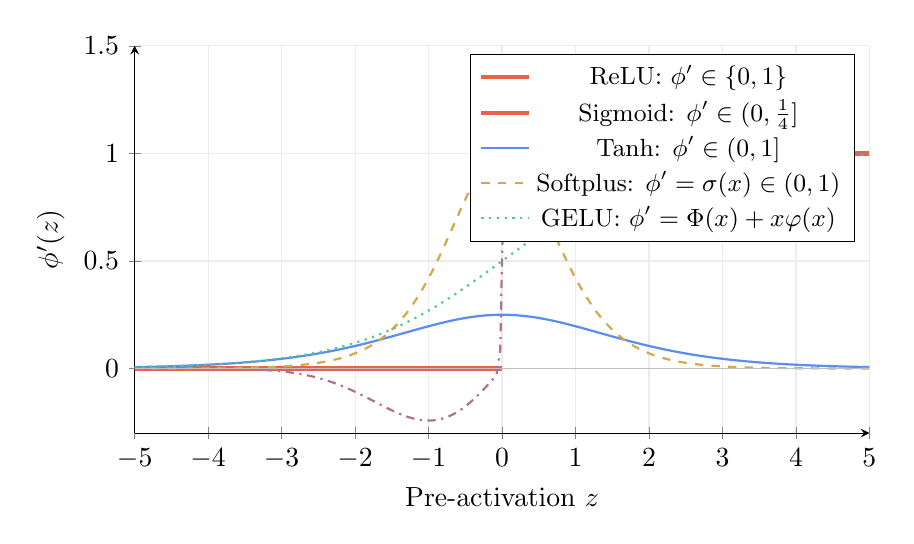
\begin{tikzpicture}
  \begin{axis}[
    width=0.9\textwidth,
    height=6.5cm,
    xlabel={Pre-activation $z$},
    ylabel={$\phi'(z)$},
    xmin=-5, xmax=5,
    ymin=-0.3, ymax=1.5,
    grid=major,
    grid style={gray!15},
    axis lines=left,
    legend style={at={(0.98,0.98)}, anchor=north east, font=\small},
    every axis plot/.append style={thick}
  ]
  % ReLU
  \addplot[accent, ultra thick, domain=-5:0, samples=50] {0};
  \addplot[accent, ultra thick, domain=0:5, samples=50] {1};
  \addlegendentry{ReLU: $\phi' \in \{0, 1\}$}

  % Sigmoid
  \addplot[accentblue, thick, domain=-5:5, samples=200]
    {1/(1+exp(-x)) * (1 - 1/(1+exp(-x)))};
  \addlegendentry{Sigmoid: $\phi' \in (0, \frac{1}{4}]$}

  % Tanh
  \addplot[gold, thick, dashed, domain=-5:5, samples=200]
    {1 - tanh(x)^2};
  \addlegendentry{Tanh: $\phi' \in (0, 1]$}

  % Softplus = sigmoid
  \addplot[accentgreen, thick, dotted, domain=-5:5, samples=200]
    {1/(1+exp(-x))};
  \addlegendentry{Softplus: $\phi' = \sigma(x) \in (0,1)$}

  % GELU — use tanh approximation: Phi(x) ≈ 0.5*(1+tanh(sqrt(2/pi)*(x+0.044715*x^3)))
  \addplot[accent!60!accentblue, thick, dashdotted, domain=-5:5, samples=200]
    {0.5*(1+tanh(deg(sqrt(2/pi)*(x+0.044715*x^3)))) + x * exp(-0.5*x*x)/sqrt(2*pi)};
  \addlegendentry{GELU: $\phi' = \Phi(x) + x\varphi(x)$}

  % Zero line
  \addplot[gray!50, thin, domain=-5:5] {0};

  \end{axis}
\end{tikzpicture}
\caption{Derivatives $\phi'(z)$ of standard activations.  Where $\phi' = 0$, the Jacobian $\mathbf{J}_F = \mathbf{D}_\phi \mathbf{W}$ loses exact rank; where $\phi' \approx 0$ but nonzero, the Jacobian becomes ill-conditioned (effective rank shrinks without exact rank loss).  ReLU has exact zeros; sigmoid and tanh saturate smoothly toward zero; softplus remains strictly positive everywhere; GELU has a small negative dip near $z \approx -1.4$.}
\label{fig:derivatives}
\end{figure}

\begin{table}[ht]
\centering
\renewcommand{\arraystretch}{1.3}
\begin{tabular}{@{} l c c c c @{}}
\toprule
\textbf{Activation} & \textbf{Range of $\phi'$} & \textbf{Rank collapse?} & \textbf{$\phi$ injective?} & \textbf{Smooth?} \\
\midrule
Linear    & $\{1\}$          & No            & Yes  & $C^\infty$ \\
ReLU      & $\{0, 1\}$       & Yes (hard)    & No               & pw.\ $C^\infty$, not $C^1$ \\
Leaky ReLU & $\{\alpha, 1\}$ & No            & Yes              & pw.\ $C^\infty$, not $C^1$ \\
Sigmoid   & $(0, \frac{1}{4}]$ & Asymptotic  & Yes              & $C^\infty$ \\
Tanh      & $(0, 1]$         & Asymptotic    & Yes              & $C^\infty$ \\
Softplus  & $(0, 1)$         & No            & Yes              & $C^\infty$ \\
GELU      & $\approx [-0.13, 1.13]$ & Near-zero & No (non-monotone) & $C^\infty$ \\
\bottomrule
\end{tabular}
\caption{Geometric properties of standard activations.  ``Rank collapse'' distinguishes between \emph{exact} collapse ($\phi'(z) = 0$ for some $z$, as in ReLU) and \emph{asymptotic} ill-conditioning ($\phi'(z) \to 0$ but never reaches it, as in sigmoid/tanh).  ``$\phi$ injective?'' refers to whether the scalar activation is globally injective (a necessary condition for the layer to be injective).}
\label{tab:activations}
\end{table}


% ═══════════════════════════════════════════════════════════════════════════════
\section{Topological Consequences}
\label{sec:topology}
% ═══════════════════════════════════════════════════════════════════════════════

\subsection{When Is the Map a Homeomorphism?}

\begin{theorem}[Sufficient condition for topological preservation]
\label{thm:topology}
Let $F(\mathbf{x}) = \phi(\mathbf{W}\mathbf{x} + \mathbf{b})$ with $\mathbf{W} \in \mathbb{R}^{m \times n}$ and $\phi: \mathbb{R} \to \mathbb{R}$ continuous and applied coordinatewise, and let $M \subset \mathbb{R}^n$ be a compact data manifold.
If:
\begin{enumerate}[label=(\alph*)]
  \item $\mathbf{W}$ has full column rank ($\operatorname{rank}(\mathbf{W}) = n$, requiring $m \geq n$), and
  \item $\phi$ is \emph{strictly monotone} (i.e., $\phi(a) < \phi(\mathbf{b})$ whenever $a < \mathbf{b}$),
\end{enumerate}
then $F|_M: M \to F(M)$ is a homeomorphism.
Smoothness of $\phi$ is \emph{not} required---continuity and strict monotonicity suffice.
\end{theorem}

\begin{proof}
If $\mathbf{W}$ has full column rank, then $\mathbf{x} \mapsto \mathbf{W}\mathbf{x} + \mathbf{b}$ is injective.  If $\phi$ is strictly monotone, then $\phi^{-1}$ exists and $\mathbf{z} \mapsto \phi(\mathbf{z})$ is injective coordinatewise.  The composition of injectives is injective.  Since $\phi$ is continuous and strictly monotone, $F$ is a continuous injection.  A continuous injection from a compact space into a Hausdorff space is a homeomorphism onto its image (see, e.g., Munkres~\cite{munkres2000topology}, Theorem~26.6), so $F|_M$ is a homeomorphism onto $F(M)$.
\end{proof}

\begin{remark}[Necessity]
\label{rem:necessity}
The converse---that conditions (a) and (b) are \emph{necessary}---holds for the ambient map $F: \mathbb{R}^n \to \mathbb{R}^m$ but not in general for restrictions to a particular compact $M$.
If $\mathbf{W}$ is rank-deficient, then $\ker(\mathbf{W}) \neq \{0\}$, and $F(\mathbf{x}) = F(\mathbf{x}+\mathbf{v})$ for $\mathbf{v} \in \ker(\mathbf{W})$; but $\mathbf{x}$ and $\mathbf{x} + \mathbf{v}$ may not both lie on a given $M$.
Similarly, non-injectivity of $\phi$ creates collisions only at pairs of points where the pre-activations reach the colliding values, which need not occur on every $M$.
Thus, strictly monotone $\phi$ plus full-rank $\mathbf{W}$ is sufficient for any compact $M$, and necessary for $F$ to be globally injective on $\mathbb{R}^n$, but for a specific $M$ the conditions could be relaxed.
\end{remark}

\begin{remark}[Smoothness and differential geometry]
\label{rem:smoothness}
Theorem~\ref{thm:topology} guarantees topological preservation (no tearing, no folding) but says nothing about the quality of the pullback metric.
For the differential-geometric analysis of Sections~\ref{sec:jacobian}--\ref{sec:tradeoff} to apply---Jacobians, singular values, pullback metrics---we additionally need $\phi$ to be differentiable ($C^1$ or smoother).
Leaky ReLU, for example, is strictly monotone and continuous, so it preserves topology, but it is only piecewise smooth ($C^0$ at the origin), which means the Jacobian is undefined at the kink.
Within the framework of this paper: \emph{strict monotonicity governs topology; smoothness governs geometry.}
(Other analytical frameworks---Lipschitz analysis, nonsmooth geometry---can handle some of these cases differently, but the slogan captures the dichotomy for the smooth differential-geometric setting we work in.)
\end{remark}

\begin{keyresult}
Among the standard activations:
\begin{itemize}
  \item \textbf{Topologically preserving:} Linear, Leaky ReLU, Sigmoid, Tanh, Softplus (all strictly monotone).
  \item \textbf{Topologically destroying:} ReLU (the scalar activation is not injective: all negative inputs map to 0), GELU (not globally monotone; the non-monotone region is narrow, but no formal guarantee prevents pre-activations from reaching it).
\end{itemize}
However, topological preservation is necessary but not sufficient for geometric preservation.  Sigmoid and tanh preserve topology but can severely degrade metric structure through saturation.
\end{keyresult}

\subsection{The Pullback Metric Under Activation Warping}

Even when $\phi$ is invertible, the pullback metric can be severely distorted.

\begin{theorem}[Metric warping bound]
\label{thm:metric-warp}
Let $F(\mathbf{x}) = \phi(\mathbf{W}\mathbf{x} + \mathbf{b})$ with $g_N = \mathbf{I}$ (Euclidean metric on $N$).
In ambient coordinates, the pullback Gram matrix at $\mathbf{x}$ satisfies:
\begin{equation}
  g_M(\mathbf{x}) = \mathbf{W}^\top \mathbf{D}_\phi(\mathbf{z})^2 \mathbf{W}, \qquad \mathbf{z} = \mathbf{W}\mathbf{x} + \mathbf{b}.
  \label{eq:pullback-explicit}
\end{equation}
The eigenvalues of $g_M$ are bounded by:
\begin{equation}
  \min_i |\phi'(z_i)|^2 \cdot \sigma_{\min}^2(\mathbf{W}) \leq \lambda_k(g_M) \leq \max_i |\phi'(z_i)|^2 \cdot \sigma_{\max}^2(\mathbf{W}).
  \label{eq:eigenvalue-bounds}
\end{equation}
Comparing the largest eigenvalue of $g_M(\mathbf{x})$ with the smallest eigenvalue of $g_M(\mathbf{x}')$ gives a worst-case bound on relative local stretching between the two points:
\begin{equation}
  \frac{\lambda_{\max}(g_M(\mathbf{x}))}{\lambda_{\min}(g_M(\mathbf{x}'))} \leq \frac{\max_i |\phi'(z_i)|^2}{\min_j |\phi'(\mathbf{z}'_j)|^2} \cdot \kappa^2(\mathbf{W}),
  \label{eq:distortion-ratio}
\end{equation}
which can be arbitrarily large when $\phi$ saturates at one point but not the other.
This is not a canonical global distortion invariant, but it bounds how differently the map stretches infinitesimal neighborhoods at $\mathbf{x}$ versus $\mathbf{x}'$.
\end{theorem}

\begin{proof}
$g_M = \mathbf{J}_F^\top \mathbf{J}_F = (\mathbf{D}_\phi \mathbf{W})^\top (\mathbf{D}_\phi \mathbf{W}) = \mathbf{W}^\top \mathbf{D}_\phi^2 \mathbf{W}$.
Let $d_{\min}^2 = \min_i \phi'(z_i)^2$ and $d_{\max}^2 = \max_i \phi'(z_i)^2$.
Since $\mathbf{D}_\phi^2$ is positive semidefinite diagonal, we have the matrix inequality $d_{\min}^2 \, \mathbf{I} \preceq \mathbf{D}_\phi^2 \preceq d_{\max}^2 \, \mathbf{I}$, which gives:
\[
  d_{\min}^2 \, \mathbf{W}^\top \mathbf{W} \preceq \mathbf{W}^\top \mathbf{D}_\phi^2 \mathbf{W} \preceq d_{\max}^2 \, \mathbf{W}^\top \mathbf{W}.
\]
By the Courant--Fischer minimax characterization, $\lambda_k(g_M) = \min_{\dim(S)=k} \max_{\mathbf{v} \in S, \|\mathbf{v}\|=1} \mathbf{v}^\top g_M \mathbf{v}$.
Applying this to both sides of the matrix inequality yields
$d_{\min}^2 \, \lambda_k(\mathbf{W}^\top \mathbf{W}) \leq \lambda_k(g_M) \leq d_{\max}^2 \, \lambda_k(\mathbf{W}^\top \mathbf{W})$.
Since $\lambda_k(\mathbf{W}^\top \mathbf{W}) = \sigma_k^2(\mathbf{W})$, the bounds follow.
The distortion ratio bound is obtained by comparing the largest eigenvalue at $\mathbf{x}$ with the smallest at $\mathbf{x}'$.
\end{proof}

\begin{figure}[ht]
\centering
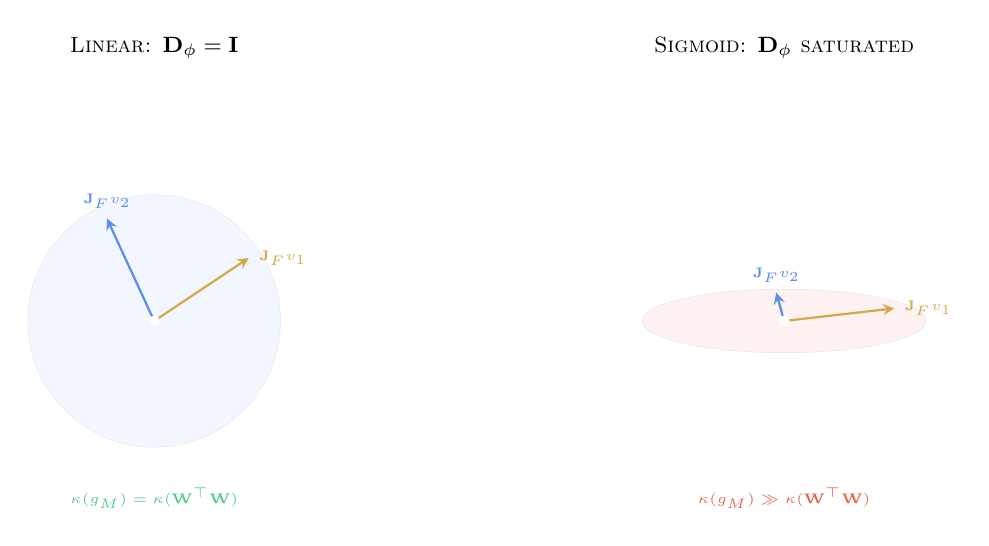
\begin{tikzpicture}[scale=2.0]
  % ── LEFT: Isometric (linear) ──
  \begin{scope}[shift={(-2.5,0)}]
    \node[font=\footnotesize\scshape, anchor=south] at (0,1.6) {Linear: $\mathbf{D}_\phi = \mathbf{I}$};

    % Unit vectors at a point
    \draw[gray!20, thin] (0,0) circle (0.8);
    \fill[accentblue!8] (0,0) circle (0.8);

    % Tangent vectors (equal length)
    \draw[gold, thick, ->, >=stealth] (0,0) -- (0.6,0.4) node[right, font=\tiny] {$\mathbf{J}_F v_1$};
    \draw[accentblue, thick, ->, >=stealth] (0,0) -- (-0.3,0.65) node[above, font=\tiny] {$\mathbf{J}_F v_2$};
    \fill[white] (0,0) circle (1pt);

    \node[font=\tiny, text=accentgreen, anchor=north] at (0,-1) {$\kappa(g_M) = \kappa(\mathbf{W}^\top \mathbf{W})$};
  \end{scope}

  % ── RIGHT: Warped (sigmoid) ──
  \begin{scope}[shift={(1.5,0)}]
    \node[font=\footnotesize\scshape, anchor=south] at (0,1.6) {Sigmoid: $\mathbf{D}_\phi$ saturated};

    % Warped ellipse
    \draw[gray!20, thin] (0,0) ellipse (0.9 and 0.2);
    \fill[accent!8] (0,0) ellipse (0.9 and 0.2);

    % Warped tangent vectors
    \draw[gold, thick, ->, >=stealth] (0,0) -- (0.7,0.08) node[right, font=\tiny] {$\mathbf{J}_F v_1$};
    \draw[accentblue, thick, ->, >=stealth] (0,0) -- (-0.05,0.18) node[above, font=\tiny] {$\mathbf{J}_F v_2$};
    \fill[white] (0,0) circle (1pt);

    \node[font=\tiny, text=accent, anchor=north] at (0,-1) {$\kappa(g_M) \gg \kappa(\mathbf{W}^\top \mathbf{W})$};
  \end{scope}
\end{tikzpicture}
\caption{The pullback metric as an ellipsoid of tangent vector lengths.
\textbf{Left:} Linear activation preserves the conditioning of $\mathbf{W}$.
\textbf{Right:} Sigmoid saturation compresses one axis dramatically, worsening the condition number and distorting distances.}
\label{fig:metric-warp}
\end{figure}


% ═══════════════════════════════════════════════════════════════════════════════
\section{The Expressivity--Geometry Tradeoff}
\label{sec:tradeoff}
% ═══════════════════════════════════════════════════════════════════════════════

The analysis above lets us articulate a central design tension.
What follows is not a theorem but a conjectural design principle---one that the formal results to this point make plausible, but that admits sharper formulation when ``expressivity'' is given a precise definition.

\subsection{Why Activations Exist: Simulated Locality}

Without activations, a stack of $L$ layers produces a single linear map $\mathbf{W}_L \cdots \mathbf{W}_2 \mathbf{W}_1$---no increased expressivity, no ability to separate nonlinearly entangled classes.
Activations provide \emph{selectivity}: each neuron's pre-activation $z_i = \mathbf{w}_i^\top \mathbf{x} + b_i$ measures similarity to a learned prototype $\mathbf{w}_i$, and the activation $\phi$ decides which similarities to pass through.

\begin{definition}[Prototype selectivity]
The \emph{selectivity} of neuron $i$ at input $\mathbf{x}$ is $\phi'(z_i)$.
When $\phi'(z_i) \approx 0$, the neuron is ``blind'' to its prototype---it contributes no information to the downstream representation.
When $\phi'(z_i) \approx 1$, the neuron faithfully transmits its projection.
\end{definition}

This selectivity is the source of expressivity: it allows the network to implement nonlinear decision boundaries by activating different subsets of neurons in different input regions.
But it comes at a cost.

\subsection{The Tradeoff}

\begin{designprinciple}
\textbf{The expressivity--geometry tradeoff} (conjectural).
For a layer $F(\mathbf{x}) = \phi(\mathbf{W}\mathbf{x} + \mathbf{b})$:
\begin{enumerate}[label=(\roman*)]
  \item \textbf{More selectivity} $\Rightarrow$ entries of $\mathbf{D}_\phi$ closer to $\{0, 1\}$ $\Rightarrow$ sharper nonlinearity $\Rightarrow$ better separation of classes $\Rightarrow$ worse geometry (rank collapse or ill-conditioning, non-invertibility).
  \item \textbf{More geometry preservation} $\Rightarrow$ $\mathbf{D}_\phi \approx \mathbf{I}$ $\Rightarrow$ near-linear behavior $\Rightarrow$ less expressive $\Rightarrow$ better conditioning and invertibility.
\end{enumerate}
We conjecture that the optimal activation navigates this tradeoff: near-linear for inputs close to the decision boundary (where geometry matters), selective elsewhere (where expressivity matters).
This remains a design intuition rather than a formal result; making it precise would require a rigorous definition of ``expressivity'' that accounts for depth and width.
\end{designprinciple}

From the perspective developed here, GELU and softplus occupy an appealing middle ground: both are smooth, both avoid exact zeros in $\phi'$, and both transition gradually from suppression to transmission.
ReLU is a corner solution that maximizes selectivity at the cost of geometry.

\subsection{The Philosophical Point}

The tradeoff reveals something deeper: \emph{representation learning is a geometric problem}.
The goal is not merely to find features that separate classes---it is to find a map $F|_M: M \to \mathbb{R}^m$ that preserves sufficient geometric structure for downstream tasks to work.

Cosine similarity, Euclidean $k$-NN, clustering---all of these downstream operations assume that the metric structure of $N$ reflects meaningful relationships.
If the map $F$ has destroyed that structure through rank collapse or metric warping, no amount of downstream sophistication can recover it.

\begin{designprinciple}
\textbf{Task-relevant geometry must be preserved end-to-end.}
Real models often benefit from collapsing nuisance directions; the goal is not to preserve all geometry, but to preserve the structure that downstream tasks rely on.
\begin{enumerate}[label=(\alph*)]
  \item Choose activations that minimize Jacobian rank deficiency along task-relevant directions.
  \item Control input magnitudes (via normalization) to avoid saturation.
  \item Regularize the Jacobian's condition number when geometric fidelity matters (e.g., normalizing flows, metric learning).
  \item Match the evaluation metric to the geometry preserved by the network.
\end{enumerate}
\end{designprinciple}


% ═══════════════════════════════════════════════════════════════════════════════
\section{High-Dimensional Scaling}
\label{sec:highdim}
% ═══════════════════════════════════════════════════════════════════════════════

The geometric pathologies described above become dramatically worse in high dimensions.

\begin{proposition}[ReLU collapse fraction---idealized]
\label{prop:relu-fraction}
Let $\mathbf{z} \in \mathbb{R}^n$ with each $z_i$ drawn independently from a symmetric distribution (mean zero).
Then the probability that at least one coordinate is zeroed by ReLU is:
\begin{equation}
  P\bigl(\exists\, i : z_i \leq 0\bigr) = 1 - 2^{-n}.
  \label{eq:relu-prob}
\end{equation}
For $n = 768$ (a typical transformer hidden dimension), this is $1 - 2^{-768} \approx 1$.
\end{proposition}

\begin{proof}
Each coordinate is positive with probability $1/2$ by the symmetry assumption.
The events are independent, so $P(\text{all positive}) = (1/2)^n = 2^{-n}$.
\end{proof}

\begin{remark}
The independence and symmetry assumptions are idealized: in practice, the pre-activations $z_i = \mathbf{w}_i^\top \mathbf{x} + b_i$ are correlated through the shared input $\mathbf{x}$, and biases shift the distribution away from zero.
Nevertheless, the qualitative conclusion is robust: under symmetric pre-activation models the expected active fraction is $1/2$, and empirically, ReLU networks often exhibit substantial instantaneous sparsity~\cite{nair2010relu}, though the exact fraction depends on architecture, bias terms, normalization, and training.
The idealized argument captures the qualitative scaling pressure toward sparsity.
\end{remark}

\begin{remark}
This does not mean ReLU is useless in high dimensions---the network learns to route information through the active coordinates.
But it does mean that at every point, a substantial fraction of output coordinates are zeroed (\emph{sparsification}).
Whether this sparsification causes actual rank collapse depends on whether the surviving row submatrix $\mathbf{W}_{S(\mathbf{x}),:}$ retains full column rank (Theorem~\ref{thm:relu-collapse}).
When $m \gg n$, many rows can be zeroed while $\mathbf{W}_{S(\mathbf{x}),:}$ still spans $\mathbb{R}^n$; when $m \approx n$, sparsification and rank collapse are closely linked.
\end{remark}

\begin{proposition}[Expected active fraction]
For the setup of Proposition~\ref{prop:relu-fraction}, the expected fraction of active coordinates is exactly $1/2$, and the standard deviation of the active fraction is $O(n^{-1/2})$.
Thus for large $n$, almost exactly half the coordinates are zeroed at every point.
\end{proposition}

\begin{figure}[ht]
\centering
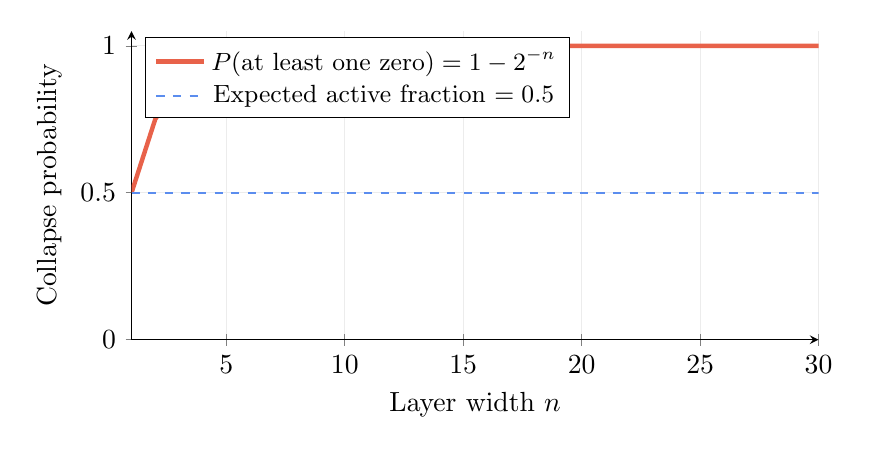
\begin{tikzpicture}
  \begin{axis}[
    width=0.85\textwidth,
    height=5.5cm,
    xlabel={Layer width $n$},
    ylabel={Collapse probability},
    xmin=1, xmax=30,
    ymin=0, ymax=1.05,
    grid=major,
    grid style={gray!15},
    axis lines=left,
    legend style={at={(0.02,0.98)}, anchor=north west, font=\small}
  ]
  \addplot[accent, ultra thick, domain=1:30, samples=30]
    {1 - (0.5)^x};
  \addlegendentry{$P(\text{at least one zero}) = 1 - 2^{-n}$}

  \addplot[accentblue, thick, dashed, domain=1:30, samples=30]
    {0.5};
  \addlegendentry{Expected active fraction $= 0.5$}

  \addplot[only marks, mark=*, mark size=2pt, gold] coordinates {(10,0.999)};
  \node[gold, font=\footnotesize, anchor=south west] at (axis cs:10.5,0.93) {$n=10$: 99.9\%};

  \end{axis}
\end{tikzpicture}
\caption{In $n$ dimensions (under the idealized iid symmetric model), the probability that ReLU zeros at least one coordinate approaches 1 exponentially fast.
By $n = 10$, it is already 99.9\%.  The expected active fraction is always 50\%.
Under these assumptions, approximately half the rows of $\mathbf{J}_F$ are zeroed at any point; whether this translates to rank loss depends on the structure of the surviving submatrix $\mathbf{W}_{S(\mathbf{x}),:}$.}
\label{fig:highdim}
\end{figure}


\subsection{Multi-Layer Composition}

The single-layer analysis extends naturally to deep networks.
For an $L$-layer network $F = F_L \circ \cdots \circ F_1$ with $F_\ell(\mathbf{x}) = \phi(\mathbf{W}_\ell \mathbf{x} + \mathbf{b}_\ell)$, the chain rule gives:
\begin{equation}
  \mathbf{J}_F(\mathbf{x}) = \prod_{\ell=L}^{1} \mathbf{D}_{\phi}(\mathbf{z}^{(\ell)}) \, \mathbf{W}_\ell,
  \label{eq:deep-jacobian}
\end{equation}
where $\mathbf{z}^{(\ell)}$ is the pre-activation at layer $\ell$.
Rank defects \emph{compound}: if $\mathbf{D}_{\phi}(\mathbf{z}^{(\ell)})$ drops $k_\ell$ dimensions at layer $\ell$, the end-to-end rank satisfies $\operatorname{rank}(\mathbf{J}_F) \leq \min_\ell \operatorname{rank}(\mathbf{D}_{\phi}(\mathbf{z}^{(\ell)}) \mathbf{W}_\ell)$.
For ReLU networks, this means the effective dimension of the representation can only decrease or stay the same through depth---geometry lost at any layer is lost permanently.
This compounding effect is a key motivation for residual connections~\cite{he2015resnet}, which bias the Jacobian toward $\mathbf{I} + \text{(perturbation)}$ and can mitigate---though not guarantee prevention of---cumulative degeneracy in very deep networks.
The complementary architectural strategy of \emph{enforcing} invertibility, through unitary parameterizations~\cite{arjovsky2016unitary} or invertible residual networks~\cite{behrmann2019invertible}, removes the rank-loss failure mode at the cost of additional constraints on $\mathbf{W}$.
A related strand of analysis studies the spectral and expressive geometry of deep networks under standard activations~\cite{montufar2014number,poole2016exponential,pennington2018emergence,raghu2017svcca}.

% ═══════════════════════════════════════════════════════════════════════════════
\section{Discussion: Activations as Geometry}
\label{sec:deeper}
% ═══════════════════════════════════════════════════════════════════════════════

\subsection{The Map Is the Representation}

A representation is not a set of features---it is a \emph{map} $F|_M: M \to \mathbb{R}^m$.
The quality of the representation is the quality of this map: does it preserve the geometric structure needed for downstream tasks?

\begin{remark}[Standard techniques as Jacobian regularization]
This perspective reframes several standard deep learning practices as forms of Jacobian regularization:
\textbf{(i)}~Residual connections add $\mathbf{x}$ to $F(\mathbf{x})$, keeping the Jacobian near $\mathbf{I} + \mathbf{J}_{\text{branch}}$ and helping mitigate degeneracy.
\textbf{(ii)}~Batch normalization rescales activations to prevent saturation, keeping $\mathbf{D}_\phi$ away from zero.
\textbf{(iii)}~Layer normalization constrains representations to near a sphere, connecting to geometry-objective alignment.
\textbf{(iv)}~Skip and dense connections increase the effective rank of the end-to-end Jacobian.
A full treatment of these connections is beyond the scope of this paper, but the pattern is consistent: techniques that stabilize training also stabilize the geometry of the learned map.
\end{remark}

\subsection{The Riemannian View}

If we equip the representation space $N$ with the standard Euclidean metric, the pullback induced by the restricted differential is a Riemannian metric on $M$ wherever $d(F|_M)_{\mathbf{x}}$ is injective.
This metric encodes the network's ``belief'' about which data points are close and which are far.

\begin{geometricinsight}
The optimal learned metric $g_M^*$ should satisfy:
\begin{itemize}
  \item Points from the same class should have small geodesic distance under $g_M^*$.
  \item Points from different classes should have large geodesic distance under $g_M^*$.
  \item The metric should be smooth and well-conditioned (no singularities or degeneracies).
\end{itemize}
Activations that cause rank collapse create degeneracies in the pullback metric, where the Riemannian description breaks down and distances along some directions collapse.
\end{geometricinsight}

\subsection{Implications for Evaluation Metrics}

This geometric perspective connects directly to our earlier work on cosine similarity~\cite{bouhsine2026cosine}.
If the network's Jacobian is well-conditioned, then cosine similarity in representation space reflects genuine angular relationships on the data manifold.
If the Jacobian has collapsed, cosine similarity in representation space is comparing artifacts, not features.

\begin{keyresult}
\textbf{The full pipeline.}  For cosine similarity to be meaningful:
\begin{enumerate}[label=(\roman*)]
  \item Train with normalization (so the gauge freedom doesn't arise).
  \item Use activations that preserve Jacobian rank (so the map doesn't destroy geometry).
  \item Control input magnitudes (so activations don't saturate).
\end{enumerate}
Condition (i) was the subject of our companion paper.  Conditions (ii) and (iii) are the subject of this one.
\end{keyresult}


\paragraph{Summary.}
The mathematical content of the paper is compact enough to fit in a single table.

\begin{table}[ht]
\centering
\renewcommand{\arraystretch}{1.3}
\begin{tabular}{@{} p{5.5cm} p{5.5cm} @{}}
\toprule
\textbf{Concept} & \textbf{Formal statement} \\
\midrule
Layer Jacobian &
$\mathbf{J}_F = \mathbf{D}_\phi(\mathbf{z}) \cdot \mathbf{W}$: diagonal modulation of the linear map \\[4pt]
Exact rank collapse (ReLU) &
$\operatorname{rank}(\mathbf{J}_F) = \operatorname{rank}(\mathbf{W}_{S(\mathbf{x}),:})$ where $S(\mathbf{x}) = \{i : z_i > 0\}$ \\[4pt]
Ill-conditioning (sigmoid, tanh) &
$\phi'(z_i) \to 0$ degrades $\kappa(\mathbf{J}_F)$ without exact rank loss \\[4pt]
Volume collapse &
$\mathrm{vol}_n(\mathbf{J}_F) = 0$ when $\operatorname{rank}(\mathbf{J}_F) < n$ (exact, e.g.\ ReLU); $\mathrm{vol}_n(\mathbf{J}_F) \to 0$ under saturation \\[4pt]
Pullback metric &
$g_M = \mathbf{W}^\top \mathbf{D}_\phi^2 \mathbf{W}$: activation warps distances \\[4pt]
Topological preservation &
Sufficient: $\phi$ strictly monotone $+$ $\mathbf{W}$ full column rank \\[4pt]
High-dim collapse (ReLU) &
$P(\text{at least 1 dead neuron}) = 1 - 2^{-n}$ \\
\bottomrule
\end{tabular}
\caption{Summary of the geometric analysis of activation functions.}
\label{tab:summary}
\end{table}

\begin{keyresult}
Activations are not nonlinearities added for expressivity and then forgotten.
They are \textbf{geometric operators} that control the Jacobian, the pullback metric, and the topology of the learned representation.
When they are many-to-one and induce zero derivatives (ReLU), the Jacobian may lose exact rank and information along the killed directions is destroyed.
When they saturate (sigmoid, tanh), exact rank is preserved but the Jacobian becomes ill-conditioned: effective dimension shrinks and metric structure is distorted.
When they are non-smooth ($C^0$ only), the Jacobian is undefined at the non-differentiable points, and the differential-geometric framework simply does not apply there.

The decomposition to keep in mind is
\[
  \underbrace{F = \phi \circ (\mathbf{W} \cdot {+}\, \mathbf{b})}_{\text{layer}}, \qquad
  \mathbf{J}_F = \underbrace{\mathbf{D}_\phi}_{\text{geometric modulation}} \;\cdot\; \underbrace{\mathbf{W}}_{\text{learned geometry}}.
\]
Choose the activation with the same care you choose the loss; both decide the geometry of the representation.
\end{keyresult}


% ─── REFERENCES ────────────────────────────────────────────────────────────────
\begin{thebibliography}{9}

\bibitem{bengio2013manifold}
Y.~Bengio, A.~Courville, and P.~Vincent.
\newblock Representation learning: A review and new perspectives.
\newblock \emph{IEEE TPAMI}, 35(8):1798--1828, 2013.

\bibitem{bouhsine2026cosine}
T.~Bouhsine.
\newblock In defense of cosine similarity: Normalization eliminates the gauge freedom.
\newblock \emph{arXiv preprint arXiv:2602.19393}, 2026.
\newblock \url{https://arxiv.org/abs/2602.19393}

\bibitem{hendrycks2016gelu}
D.~Hendrycks and K.~Gimpel.
\newblock Gaussian error linear units (GELUs).
\newblock \emph{arXiv preprint arXiv:1606.08415}, 2016.

\bibitem{he2015resnet}
K.~He, X.~Zhang, S.~Ren, and J.~Sun.
\newblock Deep residual learning for image recognition.
\newblock In \emph{Proc.\ CVPR}, 2016.

\bibitem{arjovsky2016unitary}
M.~Arjovsky, A.~Shah, and Y.~Bengio.
\newblock Unitary evolution recurrent neural networks.
\newblock In \emph{Proc.\ ICML}, 2016.

\bibitem{behrmann2019invertible}
J.~Behrmann, W.~Grathwohl, R.~T.~Q.~Chen, D.~Duvenaud, and J.-H.~Jacobsen.
\newblock Invertible residual networks.
\newblock In \emph{Proc.\ ICML}, 2019.

\bibitem{nair2010relu}
V.~Nair and G.~E.~Hinton.
\newblock Rectified linear units improve restricted Boltzmann machines.
\newblock In \emph{Proc.\ ICML}, 2010.

\bibitem{montufar2014number}
G.~Mont\'{u}far, R.~Pascanu, K.~Cho, and Y.~Bengio.
\newblock On the number of linear regions of deep neural networks.
\newblock In \emph{Proc.\ NeurIPS}, 2014.

\bibitem{poole2016exponential}
B.~Poole, S.~Lahiri, M.~Raghu, J.~Sohl-Dickstein, and S.~Ganguli.
\newblock Exponential expressivity in deep neural networks through transient chaos.
\newblock In \emph{Proc.\ NeurIPS}, 2016.

\bibitem{pennington2018emergence}
J.~Pennington, S.~Schoenholz, and S.~Ganguli.
\newblock The emergence of spectral universality in deep networks.
\newblock In \emph{Proc.\ AISTATS}, 2018.

\bibitem{raghu2017svcca}
M.~Raghu, J.~Gilmer, J.~Yosinski, and J.~Sohl-Dickstein.
\newblock {SVCCA}: Singular vector canonical correlation analysis for deep learning dynamics and interpretability.
\newblock In \emph{Proc.\ NeurIPS}, 2017.

\bibitem{munkres2000topology}
J.~R.~Munkres.
\newblock \emph{Topology}.
\newblock Prentice Hall, 2nd edition, 2000.

\end{thebibliography}

\end{document}
